%%%%%%%%%%%%%%%%%%%%%%%%%%%%%%%%%%%%%%%%%%%%%%%%%%%%%%%%%%%%%%%%%%%%%%%%%%%%%%%%
%2345678901234567890123456789012345678901234567890123456789012345678901234567890
%        1         2         3         4         5         6         7         8

\documentclass[letterpaper, 10 pt, conference]{ieeeconf}  % Comment this line out if you need a4paper

%\documentclass[a4paper, 10pt, conference]{ieeeconf}      % Use this line for a4 paper

\IEEEoverridecommandlockouts                              % This command is only needed if 
                                                          % you want to use the \thanks command

\overrideIEEEmargins                                      % Needed to meet printer requirements.
\usepackage{cite}
\usepackage{amsmath,amssymb,amsfonts}
\usepackage{graphicx}
\usepackage{textcomp}
\usepackage{xcolor}
\usepackage{bm}
\usepackage{float}
\usepackage{subcaption}
\usepackage{siunitx}

%\usepackage[ruled]{algorithm2e}
\usepackage{algorithm, algpseudocode}
%\SetKwComment{Comment}{$\triangleright$ }{}
\usepackage{tabu}
\usepackage{booktabs}
\usepackage{etoolbox}
\usepackage{hyperref}
\usepackage{todonotes}
\usepackage{svg}
\def\BibTeX{{\rm B\kern-.05em{\sc i\kern-.025em b}\kern-.08em
		T\kern-.1667em\lower.7ex\hbox{E}\kern-.125emX}}
\graphicspath{ {images/} }

\newrobustcmd*{\bftabnum}{%
	\bfseries
	\sisetup{output-decimal-marker={\textmd{.}}}%
}

%In case you encounter the following error:
%Error 1010 The PDF file may be corrupt (unable to open PDF file) OR
%Error 1000 An error occurred while parsing a contents stream. Unable to analyze the PDF file.
%This is a known problem with pdfLaTeX conversion filter. The file cannot be opened with acrobat reader
%Please use one of the alternatives below to circumvent this error by uncommenting one or the other
%\pdfobjcompresslevel=0
%\pdfminorversion=4

% See the \addtolength command later in the file to balance the column lengths
% on the last page of the document

% The following packages can be found on http:\\www.ctan.org
%\usepackage{graphics} % for pdf, bitmapped graphics files
%\usepackage{epsfig} % for postscript graphics files
%\usepackage{mathptmx} % assumes new font selection scheme installed
%\usepackage{times} % assumes new font selection scheme installed
%\usepackage{amsmath} % assumes amsmath package installed
%\usepackage{amssymb}  % assumes amsmath package installed

\title{\LARGE \bf
	Learning When to Fail: Contingency Plans for Crowd Navigation
}


\author{Patrick Naughton$^{1}$, Ishani Chatterjee$^{2}$, Tushar Kusnur$^{3}$, and Maxim Likhachev$^{4}$% <-this % stops a space
\thanks{Some text}% <-this % stops a space
\thanks{$^{1}$Notes
        {\tt\small patrickrnaughton@wustl.edu}}%
\thanks{$^{2}$Ishani notes
        {\tt\small ichatter@andrew.cmu.edu}}%
}


\begin{document}

\newcolumntype{Z}{S[
	table-format=1.2,% added
	%tight-spacing=true,
	round-mode=places,
	round-precision=2]}


\maketitle
\thispagestyle{empty}
\pagestyle{empty}


%%%%%%%%%%%%%%%%%%%%%%%%%%%%%%%%%%%%%%%%%%%%%%%%%%%%%%%%%%%%%%%%%%%%%%%%%%%%%%%%
\begin{abstract}
	When navigating in the presence of humans, mobile robots need robust, efficient ways of dealing with highly stochastic dynamic obstacles. This problem is often addressed by building a (implicit or explicit) model of possible human trajectories and planning the robot's motion based on this model to avoid collisions. We call this a \textit{success controller}. However, such controllers typically assume that their goal is feasible, without considering cases in which humans may move to block the robot's path. This can lead to the robot simply stopping, continuously replanning to an infeasible goal, or, in the worst case, colliding with a pedestrian. This work seeks to explicitly address this deficiency by creating a classifier that examines the robot's trajectory to determine whether or not it believes the robot can efficiently achieve its goal point. Additionally, we develop a \textit{failure controller} that the robot executes if the classifier determines that it cannot reach its goal. This controller safely guides the robot to a different location from which it can replan. We show that this failure controller results in fewer intrusions near people in a crowded scene than simply relying on the success controller.
\end{abstract}


%%%%%%%%%%%%%%%%%%%%%%%%%%%%%%%%%%%%%%%%%%%%%%%%%%%%%%%%%%%%%%%%%%%%%%%%%%%%%%%%
\section{INTRODUCTION}
	Pedestrian crowds present a challenging navigation environment for a mobile robot. The robot must comply with latent social rules governing its trajectory while simultaneously reaching its goal in a reasonable amount of time. As robots move into closer contact with humans, advanced methods for navigation in crowds will gain increased importance. Probabilistic planners, which make navigation plans in the belief space, show potential to make headway in this problem and have demonstrated success dealing with uncertainty \cite{ppcp} like that experienced navigating in a crowd. To form their plans, these planners rely on smaller atomic actions which are strung together to form an overall trajectory. Some of these actions are learned by presenting the robot with its starting pose and a waypoint pose and running simulations with pedestrians or other agents \cite{crowdawarerl}. In general, these controllers guiding each action deal with unexpected situations in which their original trajectory to their waypoint becomes infeasible by simply replanning or stopping altogether. Replanning in some cases may take too long to avoid an imminent collision. Additionally, when the waypoint becomes completely unreachable, replanning or stopping may result in a more costly trajectory than simply abandoning it and seeking a safe location from which the higher level planner can generate a new trajectory to the overall goal. We address this issue by developing a failure controller aimed explicitly at motion control for the robot when it has no goal.
	
	Developing such a controller is useful because it gives long term planners a contingency plan at planning time so they can more efficiently explore the search space. The failure controller itself also helps ensure that the robot obeys a safe policy even when it has no waypoint to navigate to. For example, in some situations like that in Figure \ref{fig:dnmotivation}, staying still will cause the robot to be a hindrance to the humans and it will likely intrude into their personal space. Moving away to a different area of the scene would give the robot a safer place to replan from.
	
	\begin{figure}
		\centering
		\begin{subfigure}[t]{0.49\linewidth}
			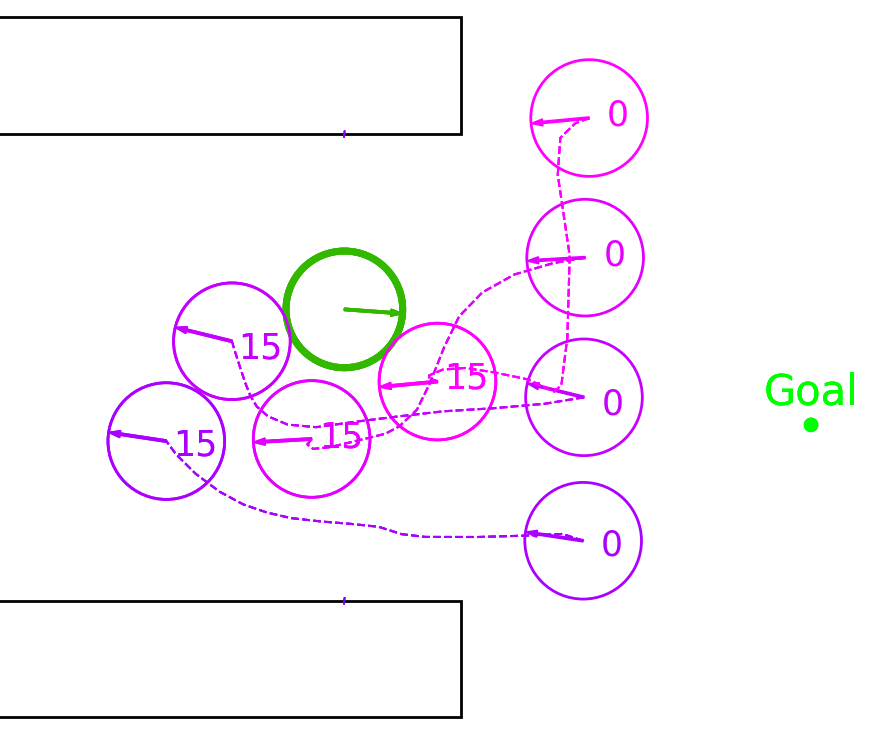
\includegraphics[width=\linewidth]{dnmotive}
			\caption{}
			\label{fig:dnmotivation}
		\end{subfigure}
		\begin{subfigure}[t]{0.49\linewidth}
			% \includegraphics{}
			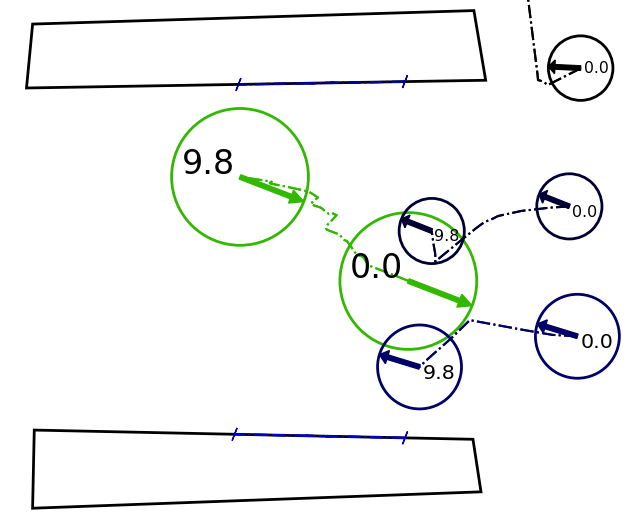
\includegraphics[width=\linewidth]{rlmotive}
			\caption{}
		\end{subfigure}
		\caption{The green circle represents the robot, the blue circles represent different humans and the black polygons represent the walls of the corridor. The arrows indicate the heading of each agent. Only the initial and final locations of each object are shown. The numbers indicate the time step at which the snapshot was taken. This is an example of a situation in which the robot stopping (a) will cause more collisions and intrusions than following a failure controller which in this case simply moves the robot along the corridor out of the way of humans (b).}
		\label{fig:motivation}
	\end{figure}
	
	This work facilitates combining learning with planning for long term crowd navigation by providing a reinforcement learning based failure controller and a supervised learning based predictor for determining when to use it. Specifically, this paper assumes that an existing probabilistic planner uses a set of motion primitives and controllers to create navigation plans. The set of controllers includes some to execute complex behaviors that interact with pedestrians. Each of these controllers has some probability of success which is associated with one goal and trajectory, and some probability of failure which is associated with a different trajectory. Success cannot be guaranteed for the controllers because the surrounding humans may interact with the robot or each other in unexpected ways. Note that the failure controller's objective differs from that of a traditional navigation planner in that the failure controller is not given an explicit goal; rather, it attempts to extract the optimal goal and trajectory from its environment.

	The contributions of this work are:
	\begin{enumerate}
		\item A classifier that determines whether or not a robot is likely to reach its goal in a given scene.
		\item A failure controller that safely guides the robot to a stable position from which it can initiate replanning.
	\end{enumerate}
	The design philosophy taken by this approach separates controllers for individual actions from the long term planner. This means the results presented here could easily be adapted to work with any planner.
	
	The remainder of this paper is organized as follows. Section \ref{sec:relatedwork} describes previous work related to the results presented here. Section \ref{sec:problemstatement} outlines our problem statement in more detail. Section \ref{sec:approach} describes our approach and Section \ref{sec:experiments} describes the experiments we performed to evaluate our design. Section \ref{sec:results} describes and discusses the results of these experiments and we conclude with Section \ref{sec:conclusion} and discuss future work.
	
	The code of our approach is available here: \texttt{\url{https://github.com/patricknaughton01/LearnController}}.
	

\section{RELATED WORK}\label{sec:relatedwork}
	Several methods use explicit models of human behavior to achieve smooth, predictable robot navigation among pedestrians. Trautman et al. model the interaction between the robot and pedestrians as an extension of an interactive Gaussian process that accommodates multiple goals \cite{caseforcoop}. The social forces model treats humans and the robot in question as masses subject to Newtonian dynamics and applies fictitious forces to them to predict and plan trajectories \cite{sfm}. It recomputes these forces and their effects on robot motion at each time step to determine how the robot should move. These techniques however rely on hand-crafted models of human behavior to achieve their results and handle unexpected or uncooperative human actions by simply replanning using the same model. The social forces model in particular does not demonstrate robust navigation plans and will sometimes exhibit oscillatory behavior in more crowded or narrow areas \cite{sfm}.
	
	Another approach uses inverse reinforcement learning to learn latent, possibly stochastic social rules humans observe when navigating in crowds \cite{socialirl}. This method uses example trajectories recorded from humans or gathered from teleoperated runs. This approach however is extremely unlikely to observe failed trajectories where a human attempts to execute some navigation plan and is forced to completely abort their initial goal. If a human attempts to overtake someone else, for example, they have many contingency options in the case where the other person is either intentionally or unintentionally uncooperative. For example, they could use verbal communication or body language to more explicitly communicate their intentions, options which are not available to many mobile robots. For this reason, inverse reinforcement learning will likely be unable to formulate a useful model for navigation when situations such as these occur.
	
	Reinforcement learning has successfully been applied to the social robot navigation problem using a variety of different models \cite{sociallyawarerl}, \cite{crowdawarerl}. Reinforcement learning is particularly suited to this application as noted in \cite{sociallyawarerl} because it is extremely difficult to specify what the optimal action for a robot to take is, but it is comparatively easy to alert the robot when it performs a socially unacceptable or unsafe action. Previous work has focused on using reinforcement learning to develop policies that generate optimal (in terms of time) paths to a robot's goal in the presence of humans or other autonomous agents. These policies however generally assume the goal is reachable and do not make contingency plans if that assumption turns out to be incorrect. Additionally, the agent is explicitly given a goal to reach by the experimenters; we wish to navigate in the case of failure at which point there is no obvious goal.
	
	The above methods all either deal with failure at execution time by simply replanning or do not consider failure to reach the goal at all. We depart from this paradigm by designing a controller specifically targeted at producing trajectories when the robot's original goal is no longer reachable.
	
\section{PROBLEM STATEMENT}\label{sec:problemstatement}
	We consider a robot that strings together different motion primitives and controllers to generate a navigation policy to reach some overall goal. Motion primitives are basic actions the robot can take which are guaranteed to succeed, for example, drive forward one meter. Controllers are more complicated actions that may fail, for example, barging past a group of pedestrians. These controllers can be used by the robot in specific situations to navigate in a scene. We refer to the controller that guides the robot a \textit{success controller}. This work is concerned with detecting and handling the failure of these controllers. Specifically, we develop a \textit{failure controller} that corresponds to a given success controller. This failure controller directs the robot if it is determined at execution time that the success controller is unlikely to achieve its goal. 
	
	Additionally, we would like to rigorously determine at execution time whether or not the success controller is likely to succeed. In this framework, the robot can decide at each time step whether it should begin using the failure controller. Once it switches to the failure controller, it cannot switch back to the success controller until the planner generates a new plan. 
		
\section{APPROACH}\label{sec:approach}
	We begin with a fixed success controller. In this work, we consider one specific controller for barging into a group of people at the end of a corridor. While the experiments and results here only concern this controller, the framework can be extended to include other controllers as well, for example, to overtake or cross in front of pedestrians. To characterize the state of the robot, an initial matrix is constructed with the same number of rows as there are agents and obstacles in the scene (including the robot). Each row of the matrix takes the form $(d_x, d_y, s_\text{pref}, h, r, v_x, v_y, p'_x, p'_y, v'_x, v'_y, r', d, r_\text{sum})$ where 
	
	\begin{itemize}
		\item $d_x$ and $d_y$ are the $x$ and $y$ distances from the robot to the goal.
		\item $s_\text{pref}$ is the preferred speed of the robot.
		\item $h$ is the heading of the robot w.r.t. the global coordinate frame.
		\item $r$ is the radius of the robot.
		\item $v_x$ and $v_y$ are the x and y velocities of the robot w.r.t. the robot's coordinate frame.
		\item $p'_x$ and $p'_y$ are the x and y coordinates of the other agent w.r.t. the robot's coordinate frame.
		\item $v'_x$ and $v'_y$ are the x and y velocities of the other agent w.r.t. the robot's coordinate frame (note, this is not relative to the robot's velocity, just relative to its rotation).
		\item $r'$ is the radius of the other agent.
		\item $d$ is the Euclidean distance between the robot and the other agent.
		\item $r_\text{sum}$ is the sum of the radii of the robot and the other agent.
	\end{itemize}

	The first five components of each row are referred to as the robot's \verb|self_state| because they pertain specifically to the robot.
	
	This is augmented by a series of occupancy maps, one for each human and obstacle in the scene and one for the robot itself. Each occupancy map is centered on and aligned with its respective agent and their heading and is discretized into a number of squares. Each square indicates in a binary fashion whether or not it contains an object. Each square also contains the average velocity of all the objects within that square (simply set to 0 if the square is unoccupied). In our case, each occupancy map is discretized into 16 (4x4) 1 unit squares. This collection of occupancy maps and information about the robot's dynamics form the robot's \textit{state}. Note that the dimensions of the state matrix will vary depending on the number of humans and obstacles in the scene.
	
	This combined state is used as the input to a neural network. We model our architecture off of that presented in \cite{crowdawarerl} in order to handle the variable input sizes, as the input matrix changes size based on the number of people and obstacles in the scene. This architecture was shown to produce good results for robotic navigation in the presence of pedestrians in \cite{crowdawarerl}. In addition, we include an LSTM at the end of our network so that the robot can learn relationships between successive states. Figure \ref{fig:model_arch} shows the overall architecture of the model. The output of the network has five nodes which are interpreted as the $x$ and $y$ coordinates of the mean, the $x$ and $y$ standard deviations, and the correlation between $x$ and $y$ of a Gaussian distribution of the next location of the robot conditioned on its current state. At execution time, we then feed this network its current state and attempt to move to the mean of this distribution in the next time step.
	
	\begin{figure}
		\centering
		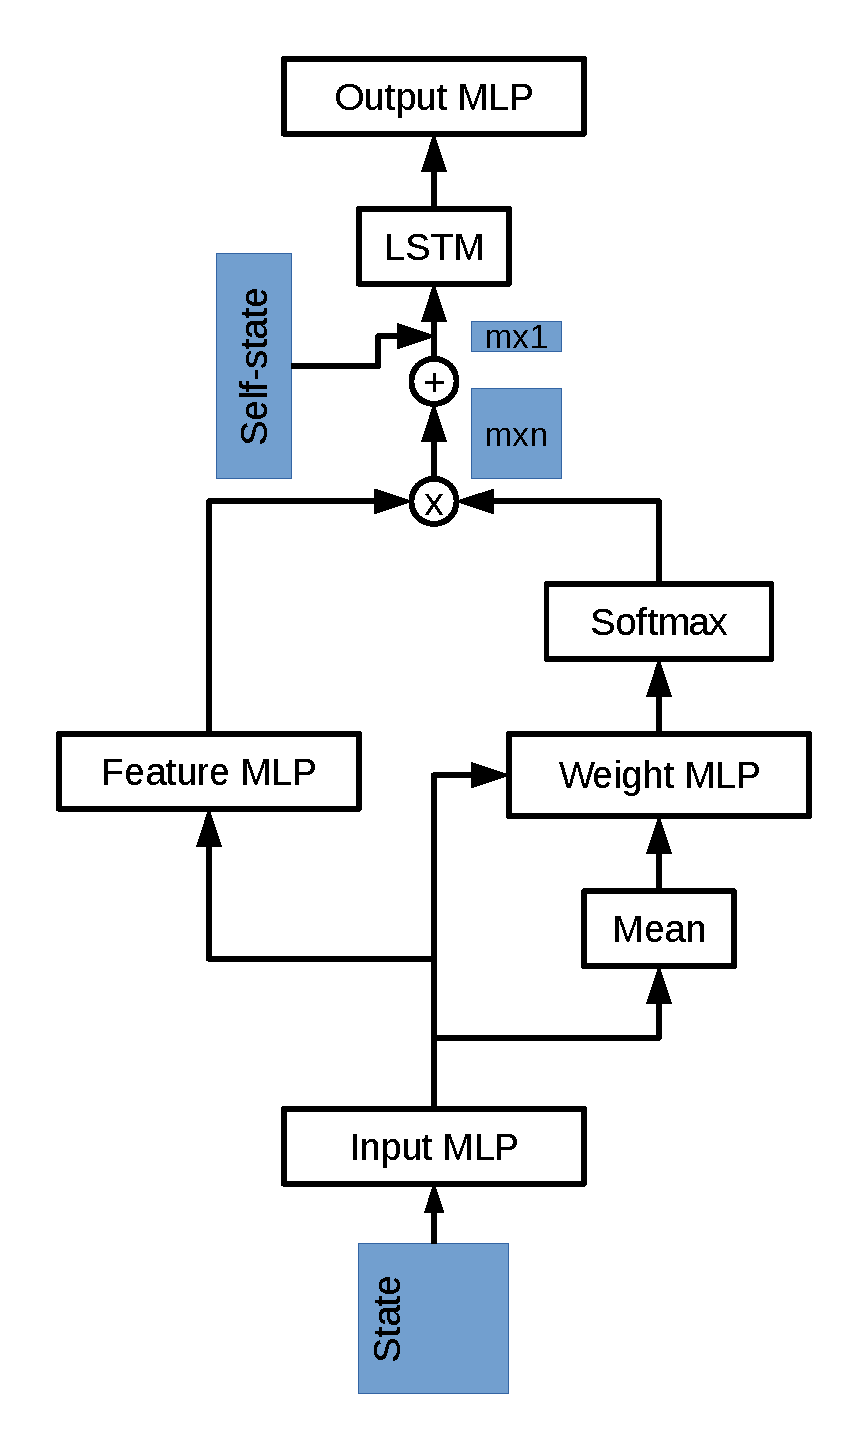
\includegraphics[height=\linewidth, angle=270]{model_arch.pdf}
		\caption{Model architecture of the neural network used to control the robot. Variable sized inputs are handled by summing a weighted vector across the people and obstacles.}
		\label{fig:model_arch}
	\end{figure}

	We trained this neural network on $1000$ successful trajectories in which the robot can feasibly reach its goal. These trajectories were generated using the RVO2 library \cite{rvo2}\cite{pyrvo2}. We trained using an Adam optimizer with a learning rate of $0.005$ and the negative 2D log-likelihood loss for $500$ epochs. This controller was trained with a very high dropout percentage of $0.5$ in each MLP. Because the success controller is not the focus of this work, we only used scenes containing four people and two obstacles. Figure \ref{fig:success} shows an example of a trajectory generated by the final controller. 

	\begin{figure}
		\centering
		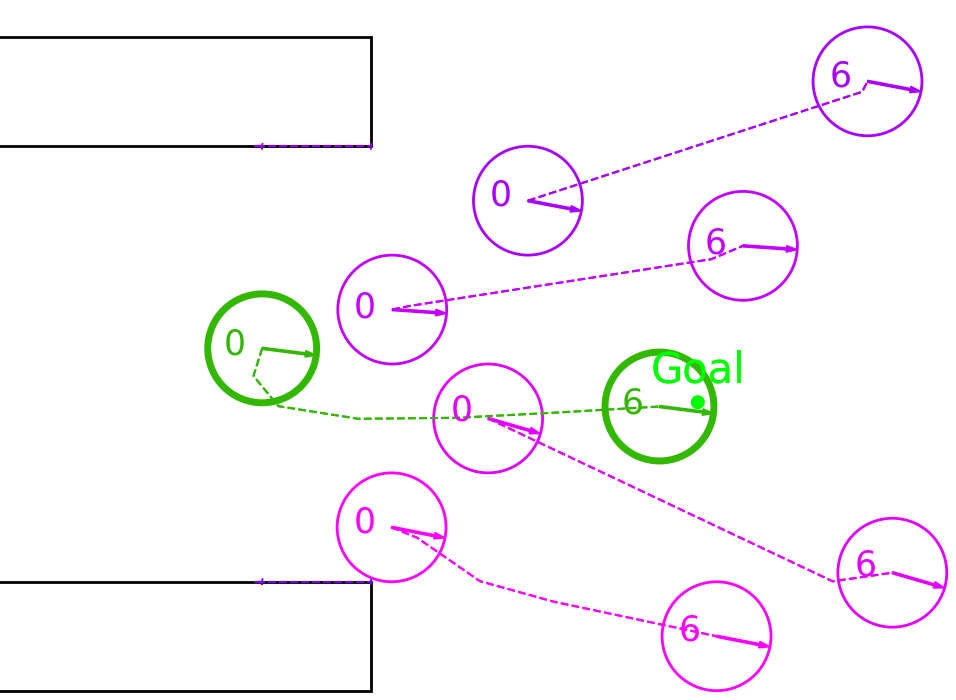
\includegraphics[width=\linewidth]{success_without_ellipses}
		\caption{Example of a successful trajectory. When executing the barge in success controller, the robot expects the humans in the scene to disperse to let it through.}
		\label{fig:success}
	\end{figure}
	
	We split the remaining approach into two distinct parts: First, we consider just determining whether or not the robot should switch to its failure controller. Given this classifier, we then develop a failure controller that, starting from the state at which the classifier reports we have failed, attempts to learn a policy that guides the robot to a safe location from which to replan.
	
	\subsection{Determining When To Switch}
		In order to rigorously determine whether or not the success controller is likely to succeed (and thus, whether or not we should switch to the failure controller), we train an additional neural network that has the same architecture as the original. However, it attempts to learn a target function that predicts the distribution of \textit{previous} locations of the robot given the robot's current state and the fact that the robot is on a trajectory that leads to its goal. It is trained on $10,000$ trajectories generated by the success controller in scenes where the success controller can reach its goal. This network however does not receive the robot's full state, rather, it only observes the robot's \textit{self state}. This was done so that we could train the network by only showing it successful trajectories without the uncertainty in its prediction exploding when it observes unsuccessful ones. 
		
		At execution time, we utilize this network's prediction to perform a statistical $p$-test with some user-specified $\alpha$ value. At each time step we construct the error ellipse given by the Gaussian distribution represented by the reverse predictor that contains $1-\alpha$ of the distribution's probability mass, and check to see if the previous robot's center is inside this ellipse. We perform this same test on the robot's current position given the distribution predicted by the success controller in the previous time step. By default, we assume that the trajectory will be successful and switch to the failure controller only if one of these tests fails.
		
		\begin{figure}
			\centering
			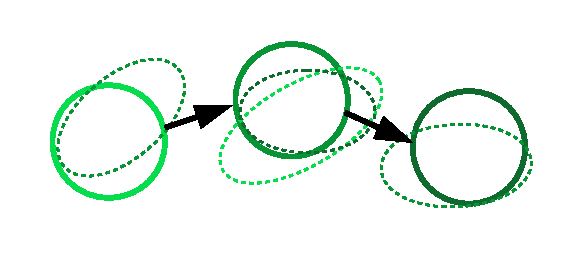
\includegraphics[width=\linewidth]{success_ellipses}
			\caption{Example of the error ellipses used to classify trajectories as successes or failures. Each shade of green is a different time step and the ellipses associated with a given time step are the same color as the robot in that step. Note that in the first and last states there are no previous or next states so these two positions only need to satisfy one test.}
		\end{figure}
	
		We employ this strategy so that we can train the reverse predictor by showing it only successful trajectories. This is desirable for two reasons. First, there are generally many fewer ways for a robot to successfully reach its goal when interacting with pedestrians than for it to fail. By only training on success trajectories, we do not have to find or generate training data for all of these potential methods of failure. Second, it is much easier to find examples of actual humans successfully barging into a group than examples of them failing to do this. This means that only using successful examples as training data will make this system better able to utilize real world human trajectories in the future.
	
	\subsection{Failure Controller}
		For the failure controller, we need to address a somewhat novel formulation of the navigation problem in that the robot now has no specific goal it is trying to reach. Once the failure controller gets invoked, the robot has determined that it is unlikely to reach its goal. Because it is impossible to explicitly define optimality in this framework, we formulate this as a reinforcement learning problem $\langle\mathcal{S}, \mathcal{A}, \mathcal{R}, \mathcal{P}, \gamma\rangle$ with an infinite set of states $\mathcal{S}$, a finite set of actions $\mathcal{A}$, state transition matrix $\mathcal{P}(s_t, a_t, s_{t+1})$, reward function $\mathcal{R}(s_t, a_t, s_{t+1})$ and discount factor $\gamma \in (0, 1)$ \cite{suttonandbarto} and model the robot as a Markovian agent. Rather than define a set of states constituting a goal, we define a reward function that punishes actions we determine to be undesirable. 
		
		Our reward function is split into three parts: $\mathcal{R}_{\text{collision}}$, $\mathcal{R}_{\text{movement}}$, and $\mathcal{R}_{\text{smoothness}}$. The overall reward the robot observes is simply the sum of these three components. Equations \ref{eq:rcollision}, \ref{eq:rmovement}, and \ref{eq:rmovement} show how these values are calculated. Note that each term is computed (where appropriate) with respect ot each agent and obstacle in the scene. This means that an action that causes a collision with two agents receives a collision reward of $-2$, not just $-1$. We apply the $\mathcal{R}_{\text{movement}}$ and $\mathcal{R}_{\text{smoothness}}$ rewards so that, other things equal, the robot will prefer to remain stationary and move in straight lines at consistent velocities that are more predictable for other humans in the scene.
		
		\begin{equation}\label{eq:rcollision}
			\mathcal{R}_{\text{collision}} = \begin{cases}
				-1      &   d < 0\\
				-0.25   &   0 \leq d < 0.2\\
				0       &   else
			\end{cases}
		\end{equation}
		
		\begin{equation}\label{eq:rmovement}
			\mathcal{R}_{\text{movement}} = \begin{cases}
			0       &   a_t = 0 \quad(remain\;still)\\
			-0.01   &   else
			\end{cases}
		\end{equation}
		
		\begin{equation}\label{eq:rsmoothness}
			\mathcal{R}_{\text{smoothness}} = \begin{cases}
			0       &   a_t = a_{t-1} \vee a_{t-1} = 0\\
			-0.01   &   else
			\end{cases}
		\end{equation}
		
		We then define a $Q_{\pi}(a_t, s_t)$ function that represents the total expected discounted return achieved by executing action $a_t$ from state $s_t$ and thereafter following policy $\pi$. 
		
		\begin{equation}\label{eq:q}
			Q_{\pi} = 
			\sum_{k=0}^{\infty}E[\gamma^k \mathcal{R}(s_{t+k}, \pi(a_{t+k} \mid s_{t+k}), s_{t+k+1})]
		\end{equation}
		
		We represent this function with a deep neural network and use the Deep Q-learning algorithm with experience replay developed in \cite{dqn} to obtain an estimate of the optimal $Q$ function. The state input is the same as that of the success controller and reverse predictor except that $d_x$ and $d_y$ are set to $0$ because We utilize an $\epsilon$-greedy policy with an $\epsilon$ that linearly decays from $1.0$ to $0.1$ over $4,000$ transitions. We set $\gamma=0.9$ and train using the Adam optimizer with learning rate $0.001$. 
		
		To train our agent, we ran $500$ episodes in which the robot begins by executing its success controller. However, the humans in the scene move in such a way to prevent the robot from barging in. Namely, they move into the corridor towards the robot rather than dispersing to allow it through. Once the failure classifier detects failure (or the success controller has executed for $15$ time steps), the robot begins executing an $\epsilon$-greedy policy and stores transitions in its replay buffer. We used a confidence value of $0.95$ to detect failure during training. At each time step, the reward achieved by the robot is computed and its policy is updated. After $15$ time steps, the current episode ends and another one is started. The failure controller moves for $15$ time steps regardless of how long the success controller moved or whether or not a failure was actually detected. 
		
		Algorithm \ref{algo:exec} summarizes the overall navigation policy of the robot. $t_s$ is the maximum number of time steps the success controller can run for, and $t_f$ is the same for the failure controller. Note that dropout remains on for both the success controller and reverse predictor at inference time. This is so that we can sample the networks' outputs multiple time to find the variance of their predictions and thereby estimate the network's epistemic uncertainty. This is then added to the data uncertainty which the model directly outputs \cite{gal2016uncertainty}. $S$ is the number of samples to draw from these networks when deciding where to move to next. $c$ is the confidence value to use when performing the $p$-test to determine whether or not the robot has failed. Here, $G^{(c)}(\mu, \Sigma)$ denotes an error ellipse that contains $c$ fraction of the probability mass of $\mathcal{N}(\mu, \Sigma)$. During execution, we set the $\epsilon$ of the failure controller to $0$ so that it behaves purely greedily. Additionally, after the robot (and humans in the scene) declare their goal velocities, our simulator uses the ORCA algorithm to adjust these velocities to attempt to make them safe (i.e., prevent collisions in the next time step) \cite{orca}. We use this functionality so that humans in the scene respond to the presence of the robot (although not entirely realistically).
		
		\begin{algorithm}
			%\SetAlgoLined
			%\DontPrintSemicolon
			\caption{Detect And Handle Failure}
			\label{algo:exec}
			\begin{algorithmic}
				\Function{Execute}{$t_s, t_f, S, c$}
					\State Initialize $C_s$, $P_r$, and $C_f$
					\State Initialize $F\leftarrow false$
					\For{$t=1..t_m$}
						\State Observe $s_t$
						\State Sample $S$ times from $C_s$, compute $\mu_s$ and $\Sigma_s$
						\State $G_s = \mathcal{N}(\mu_s, \Sigma_s)$
						\State Move towards $\mu_s$, observe $s_{t+1}$
						\State Sample $S$ times from $P_r$, compute $\mu_r$ and $\Sigma_r$
						\State $G_r = \mathcal{N}(\mu_r, \Sigma_r)$
						\If{$s_{t+1}\notin G^{(c)}_s \wedge s_t \notin G^{(c)}_r$}
							\State $F\leftarrow true$
							\State \textbf{break}
						\EndIf
					\EndFor
					\If{$F$}
						\For{$t=1..t_f$}
							\State Observe $s_t$
							\State Compute $\mu_f$ and $\Sigma_f$ from $C_f(s_t)$
							\State Move towards $\mu_f$
						\EndFor
					\EndIf
				\EndFunction
			\end{algorithmic}
		\end{algorithm}
		
\section{EXPERIMENTS}\label{sec:experiments}
	We began by testing the failure detection system to determine if we could accurately distinguish failure scenarios from successful ones. We began by testing how well it could identify success scenarios. We ran Algorithm \ref{algo:exec} on $1000$ new success scenarios similar to the ones the success controller learned from (we will refer to these as \textit{success scenes}) with $t_s=15, t_f=0, S=20, c=0.95$, where $t_f=0$ because we are only examining the performance of the failure detection and do not care what the robot does after this point in this experiment. 
	
	We then ran a similar experiment to determine how often the failure detector would correctly identify scenes in which the robot cannot reach its goal. To do this, we built a new scene in which the robot is extremely likely to fail and would have to make dangerous moves that could cause collisions with pedestrians to do so (we refer to these as \textit{failure scenes}). In this scene, four people move into the corridor, towards the robot, rather than dispersing to allow the robot through. We ran Algorithm \ref{algo:exec} on $1000$ such scenes using the same parameters as the corresponding experiment with success scenes.

	To evaluate the effectiveness of our overall framework, we ran two sets of experiments. In one, the reverse predictor is completely disabled so that the robot continues to execute its success controller regardless of what the people in the scene do. The episode ends after $15$ time steps or after the robot reaches its goal, whichever comes first. We set the parameters of Algorithm \ref{algo:exec} to the same values that were used in our tests of the failure detection system and ran this experiment on $1000$ failure scenes.
	
	In the other set, the robot begins by executing its success controller and only switches to the failure controller when the $p$-test performed by the reverse predictor fails. For these episodes, we set $t_s=15, t_f=5, S=20, c=0.95$ so that the failure controller has some time to improve its state after the detection system reports a failure. Note that if the failure detection system does not report a failure after $t_s$ time steps, the episode simply ends. Just as with the previous experiment, we ran this one on $1000$ failure scenes. Figure \ref{fig:experimentscomparison} shows a visual comparison between trajectories generated by the robot in the two experiments.
	
	\begin{figure}
		\centering
		\begin{subfigure}[t]{0.48\linewidth}
			\centering
			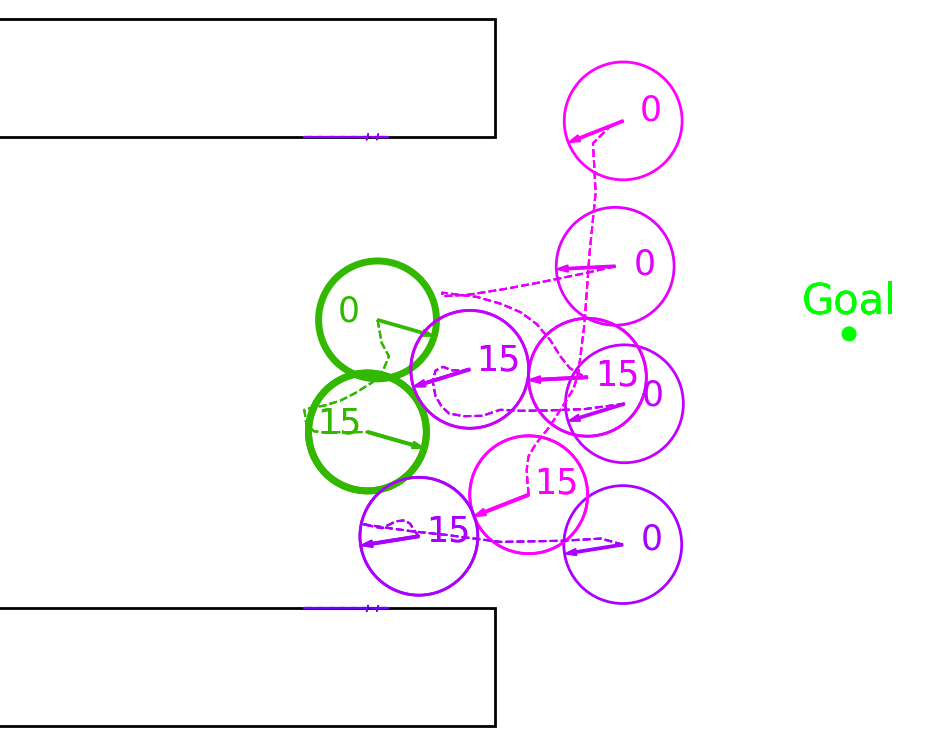
\includegraphics[width=\linewidth]{failure_without_failure_controller}
			\caption{Trajectory in which the robot continues to execute its success controller even though it incurs a very high cost to reach its goal.}
			\label{fig:failure_without_failure_controller}
		\end{subfigure}\hfill
		\begin{subfigure}[t]{0.48\linewidth}
			\centering
			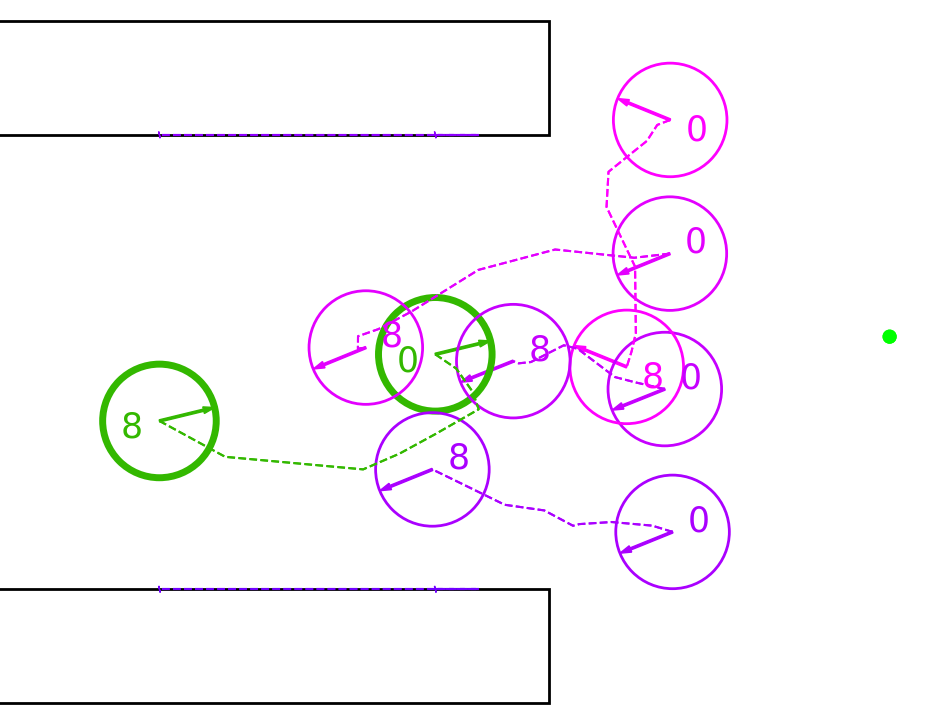
\includegraphics[width=\linewidth]{failure_with_failure_controller}
			\caption{Trajectory in which the robot realizes it cannot reach its goal and so begins executing its failure controller.}
		\end{subfigure}
		\caption{Comparison between trajectories generated by simply executing the success controller (a) versus using the failure controller when a failure is detected (b).}
		\label{fig:experimentscomparison}
	\end{figure}

\section{RESULTS}\label{sec:results}

	We found that the failure detection system reported a spurious failure in just $4$ out of the $1000$ runs on a success scene, or $0.4\%$ of the time. This result is even better than expected since we ran with $c=0.95$, meaning we would expect up to $5\%$ of these runs to be reported as failures. In failure scenes, we found that the failure detection system reported a failure in $960$ out of $1000$ runs, or $96.0\%$ of the time. This was a surprisingly positive result because neither the reverse predictor nor the success controller were ever trained on a failure trajectory. The overall accuracy of the failure detection system was $97.8\%$.
	
	To compare the overall effectiveness of the two navigation frameworks, we used versions of the metrics presented in \cite{metrics} which were designed to evaluate robot motion in crowds. These metrics are the length of the trajectory, time elapsed, angular distance traveled (computed as total change in heading between time steps), the number of collisions incurred and the number of intrusions incurred. Here, the robot is considered intruding on a human if it comes within $0.2m$ of the human. Similarly to how the reward function is computed, we count collisions (and intrusions) in each time step according to the number of humans or obstacles the robot is colliding with in that step. The time a run takes is the time from the start of the episode to when the robot last changes position. This is why all success runs do not take the full $15$ seconds and all failure runs do not take $20$ seconds. Table \ref{tab:results} summarizes these results where boldface indicates the better result. 
	
	\sisetup{
		detect-weight=true,
		detect-inline-weight=math,
		output-decimal-marker=\textnormal{.},
	}
	
	\begin{table}
		\centering
		\small
		\caption{Metrics comparing trajectories generated by a robot with no failure controller to a robot using the presented controller. The data here are averages across $1000$ runs for both cases.}\label{tab:results}
		\begin{tabu}{X[m, l] ZZ}
			\toprule
			{}&	{No Failure Controller}   & {Failure Controller (Ours)}  \\\midrule
			Length		  	&	\bftabnum 3.92&		4.64\\
			Angle		    &	\bftabnum 4.80&		6.01\\
			Time  			&	13.50&				\bftabnum 8.40\\
			Collisions  	&	0.86&				\bftabnum 0.21\\
			Intrusions  	&	15.21&				\bftabnum 6.08\\
			\midrule
		\end{tabu}
	\end{table}

	We note that the experiments without the failure controller actually achieved shorter path lengths with smaller overall changes in heading. However, as can be seen in Figure \ref{fig:failure_without_failure_controller}, this is likely because the robot simply continues to butt up against pedestrians without making much progress. Additionally, the values achieved using the failure controller are not much larger. The robot also reaches its final position faster when employing the failure controller which could potentially allow it to execute its long term navigation plans more quickly because it can begin replanning to its overall goal sooner. More importantly, using the failure controller reduces collisions by over four times and intrusions by over two times. This means that the robot behaves much more safely when it can employ the failure controller presented here rather than relying on just its success controller. 

\section{CONCLUSIONS}\label{sec:conclusion}

	This work augments the integration of learning with planning for long-term autonomous navigation. We presented a failure detection system and failure controller that allow a robot to detect when its current action is likely to fail and provide a way to safely navigate in the absence of a goal. Our failure detection system achieved a $97.8\%$ accuracy in discriminating between success and failure scenarios which was substantially better than what was expected. The use of the failure controller with the detection system also substantially reduced the number of collisions and intrusions the robot incurred when navigating in dangerous failure scenes. These contributions can allow a robot to more safely and efficiently navigate in the presence of humans by giving the robot a contingency plan in cases where it cannot execute its planned controller.
	
	In the future, we would like to extend this work to controllers for other types of situations such as crossing in front of or overtaking a pedestrian. We would also like to collect real pedestrian data from densely crowded areas such as subways and use these recorded trajectories to learn a success controller (and subsequently a reverse predictor and failure controller). These data would allow the robot to better learn how humans actually move in a given scene compared to the RVO2 simulations. This would hopefully yield navigation that is safer and more reliable than that which is currently achieved.


%\addtolength{\textheight}{-12cm}   % This command serves to balance the column lengths
                                  % on the last page of the document manually. It shortens
                                  % the textheight of the last page by a suitable amount.
                                  % This command does not take effect until the next page
                                  % so it should come on the page before the last. Make
                                  % sure that you do not shorten the textheight too much.

%%%%%%%%%%%%%%%%%%%%%%%%%%%%%%%%%%%%%%%%%%%%%%%%%%%%%%%%%%%%%%%%%%%%%%%%%%%%%%%%



%%%%%%%%%%%%%%%%%%%%%%%%%%%%%%%%%%%%%%%%%%%%%%%%%%%%%%%%%%%%%%%%%%%%%%%%%%%%%%%%



%%%%%%%%%%%%%%%%%%%%%%%%%%%%%%%%%%%%%%%%%%%%%%%%%%%%%%%%%%%%%%%%%%%%%%%%%%%%%%%%

\section*{ACKNOWLEDGMENT}
What do i put here?



%%%%%%%%%%%%%%%%%%%%%%%%%%%%%%%%%%%%%%%%%%%%%%%%%%%%%%%%%%%%%%%%%%%%%%%%%%%%%%%%

\bibliographystyle{IEEEtran}
\bibliography{ref}

\end{document}
